% 样例 1：基础三角形 + 标注（代表 80% 普通几何图）
\documentclass[tikz,border=4pt]{standalone}
\usepackage{ctex}
\usepackage{amsmath}
\usetikzlibrary{calc}
\begin{document}
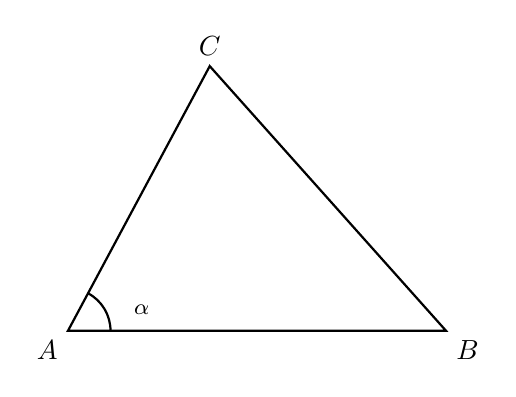
\begin{tikzpicture}[scale=1.2, thick]
  \coordinate (A) at (0, 0);
  \coordinate (B) at (4, 0);
  \coordinate (C) at (1.5, 2.8);

  \draw (A) -- (B) -- (C) -- cycle;

  \node[below left]  at (A) {$A$};
  \node[below right] at (B) {$B$};
  \node[above]       at (C) {$C$};

  % 角弧 + 标签
  \draw (0.45, 0) arc[start angle=0, end angle=62, radius=0.45];
  \node at (0.78, 0.22) {\footnotesize $\alpha$};
\end{tikzpicture}
\end{document}
